% -*- coding: utf-8; -*-
% vim: set fileencoding=utf-8 :
\documentclass[english,submission]{programming}
%% First parameter: the language is 'english'.
%% Second parameter: use 'submission' for initial submission, remove it for camera-ready (see 5.1)

\usepackage[backend=biber]{biblatex}
\addbibresource{paper.bib}

\usepackage{amsthm}
\theoremstyle{definition}
\newtheorem*{remark}{Remark}
\newtheorem*{summary}{Summary}

\usepackage{mathtools}
\usepackage{csquotes}
\usepackage{stmaryrd}
\usepackage{quiver}
\usepackage{hhline}
\usepackage{circledtext}

% define natbib citet
\newcommand{\citet}[1]{\citeauthor*{#1}~\cite{#1}}

\newcommand{\mathbox}[1]{\colorbox{black!10}{$#1$}}
\usepackage{tcolorbox}
\tcbset{colback=black!10, colframe=white, right=-20pt}

\DeclareMathOperator{\exec}{\ \fatsemi\ \ }
\newcommand{\is}{{:}\ }
\newcommand{\comma}{,\ }
\newcommand{\isa}{\dblcolon}
\newcommand{\quotedstring}[1]{\textsf{\textquotedbl{#1}\textquotedbl}}
\newcommand{\emptystring}{\textsf{\textquotedbl\ \!\textquotedbl}}
%\DeclareMathOperator{\pipe}{|}
%\DeclareMathOperator{\at}{\textsf{@}}

%%%%%%%%%%%%%%%%%%
%% These data MUST be filled for your submission. (see 5.3)
\paperdetails{
  %% perspective options are: art, sciencetheoretical, scienceempirical, engineering.
  %% Choose exactly the one that best describes this work. (see 2.1)
  perspective=art,
  %% State one or more areas, separated by a comma. (see 2.2)
  %% Please see list of areas in http://programming-journal.org/cfp/
  %% The list is open-ended, so use other areas if yours is/are not listed.
  area={Database programming, Visual and live programming, Programming environments, Version control},
  %% You may choose the license for your paper (see 3.)
  %% License options include: cc-by (default), cc-by-nc
  % license=cc-by,
}
%%%%%%%%%%%%%%%%%%

%%%%%%%%%%%%%%%%%%
%% These data are provided by the editors. May be left out on submission.
%\paperdetails{
%  submitted=2016-08-10,
%  published=2016-10-11,
%  year=2016,
%  volume=1,
%  issue=1,
%  articlenumber=1,
%}
%%%%%%%%%%%%%%%%%%


\begin{document}

\title{Baseline: Fluent Data Evolution}

\author[a]{Jonathan Edwards}[0000-0003-1958-7967]
\authorinfo{is an independent researcher interested in simplifying and democratising programming by collapsing the tech stack. He is known
for his \href{https://subtext-lang.org}{Subtext} programming language experiments and his blog at \href{https://alarmingdevelopment.org}{\texttt{alarmingdevelopment.org}}.
He has been a researcher at MIT CSAIL and CDG/HARC. He tweets \href{https://x.com/jonathoda}{\texttt{@jonathoda}} and can be reached at
\email{jonathanmedwards@gmail.com}.}
\affiliation[a]{Independent, Boston, MA, USA}

\author[b]{Tomas Petricek}[0000-0002-7242-2208]
\authorinfo{is an assistant professor at Charles University. He
is interested in finding easier and more accessible ways of thinking
about programming. To do so, he combines technical work on
programming systems and tools with research into history and
philosophy of science. His work can be found at \href{https://tomasp.net}{\texttt{tomasp.net}} and
he can be reached at \email{tomas@tomasp.net}.}
\affiliation[b]{Charles University, Prague, Czechia}


\keywords{key, word} % please provide 1--5 keywords


%%%%%%%%%%%%%%%%%%%%%%%%%%%%%
% Please go to https://dl.acm.org/ccs/ccs.cfm and generate your Classification
% System [view CCS TeX Code] stanz and copy _all of it_ to this place.
%% From HERE

% To HERE
%%%%%%%%%%%%%%%%%%%%%%%

\maketitle

\begin{abstract}

  Baseline is a platform for richly structured data supporting change in multiple dimensions: mutation over time, collaboration across space, and evolution through design changes. It is built upon \textit{Operational Differencing}, a new technique for managing data in terms of high-level operations that include refactorings and schema changes. We use operational differencing to construct an operation-based form of version control over data structures from programming languages and relational databases.

  This approach to data version control does fine-grained diffing and merging despite intervening structural transformations like schema changes. It offers users a simplified conceptual model of version control: There is no repo; Branching is just copying. The informaton maintained in a repo can be synthesized more precisely from the append-only histories of branches. Branches can be flexibly shared like spreedsheet files, except with the added benefit of diffing and merging.

  We conjecture that queries can be \textit{operationalized} into a sequence of schema and data operations. We develop that idea into a query language fragment containing selects and joins.
  Operationalized queries are represented as a \textit{future timeline} that is speculatively executed as a branch off of the present state, returning a value from its \textit{hypothetical future}. Operationalized queries get rewriten to accomodate schema change ``for free'' by the machinery of operational differencing.

  We discuss the design of Baseline's direct manipuation GUI supporting interactive schema changes as well as diffing and merging between databases.
  Altogether we develop solutions to four of the eight challenge problems of schema evolution identified in a recent paper.

\noindent\rule{\textwidth}{1pt}

% Context: What is the broad context of the work? What is the importance of the general research area?
Context: Many technologies have been developed to manage data, yet we still lack convenient general purpose tools for schema evolution and version control of data.

% Inquiry: What problem or question does the paper address? How has this problem or question been addressed by others (if at all)?
Inquiry: Can the problems of schema evolution and data version control be solved with an operation-based technique? We build upon research on Schema Modification Operations and Operational Transformation.

% Approach: What was done that unveiled new knowledge?
Approach: Most tools for data management are state-based, for pragamtic reasons of interoperability. We are exploring what is possible with an operation-based approach.

% Knowledge: What new facts were uncovered? If the research was not results oriented, what new capabilities are enabled by the work?
Knowledge: Operational Differencing is able to do fine-grained version control of data even through intervening schema changes. It can be used to synthesize more precisely the information traditionally maintained in a repo, which greatly simplifies the user's conceptual model and increases flexibility. Miller columns cen be used to visualize rich data structures. Coordinated selection can be used to visualize differences across schema changes.

% Grounding: What argument, feasibility proof, artifacts, or results and evaluation support this work?
Grounding: In prior work with others we identified eight challenge problems of schema evolution in interactive programming systems. Those challenge problems guided this research and led to solutions for four of them.
The GUI was iterated through three versions by feedback from demonstrations.

% Importance: Why does this work matter?
Importance: Our technique improves upon the known methods for schema evolution and version control of data. Our conjecture that queries can be operationalized could open up an unexplored space of query language designs.

\end{abstract}


\section{\textcolor{red}{Possible Titles}}
\textcolor{red}{
  \begin{itemize}
  \item Baseline: Fluent Data Evolution
  \item Baseline: Fluent Data Management
  \item Baseline: Operation-based Data Evolution
  \item Baseline: Operation-based Data Management
  \item Baseline: Schema Evolution and Version Control for Data
  \end{itemize}
  }


\section{Introduction}

Data changes in multiple dimensions. Data changes over time, indeed often that is the whole point. Data changes over space between replicas and variant copies. Data also changes in meaning: as needs and understanding evolve so must the shape and interpretation of the data. In practice we handle these different dimensions of change with different technologies embodying different abstractions. Programming languages, file systems, and databases all have distinct ways of managing data change over time. There are many different techniques for distributing, replicating, and collaborating on data, although surprisingly few for version control of data. There is a plethora of tools to assist in evolving the schema of databases, but in practice it often requires ad hoc programming.

Baseline is a research project to develop a general purpose mechanism for data change in all these dimensions, and to provide it conveniently to both programs and humans.
To ground this research we first surveyed one of the most problematic aspects of data change: schema evolution. In \textit{Schema Evolution in Interactive Programming Systems}~\cite{challenge-problems} we and others formulated a suite of challenge problems across a range of contexts, including traditional database programming as well as live front-end programming, model-driven development, and collaboration in computational documents.

Systems that manage change split into \textit{state-based} and \textit{operation-based} approaches~\cite{diff3, Shapiro11, edit-lenses}. State-based approaches observe only the before and after of changes, while operation-based approaches record the execution of a set of possible operations.
The benefit of state-based approaches is that since they observe from the outside they more easily interoprerate with existing tools.
The benefit of operation-based approaches is that they can capture user intentions more accurately than can be inferred from the states. For example comparing states of a table schema, a move followed by a rename is indistinguishable from a delete followed by an insert, but that makes a big difference to the data.
% We are exploring what is possible with an operation-based approach while defering the concerns of interoperability.

In this paper we introduce a new technique for operation-based change management: \textit{Operational Differencing}\textcolor{red}{ (or Operational Version Control?)}, which we define on a \textit{rich data} model curated from the features of programming languages and databases. Our contributions are:

\begin{enumerate}

\item We introduce \textit{Operational Differencing} by example in the familiar setting of typed nested lists and records supplied with a rich set of operations
including refactorings. We define the primitive transformations \textit{projection} and \textit{retraction} and the rules governing them.

\item Using these primitives we reconstruct the key features of version control: \textit{diffing} and \textit{transfer} (a specialization of merging more like cherry-picking). Because our technique is operation-based we are able to do fine-grained diffing and merging despite intervening structural transformations.

\item We simplify version control by eliminating the repo: artifacts under version control have an append-only history of operations attached to them. Branching is just making a copy of the artifact with its history, which can then diverge. There is no need for a repo to record a graph of branches and merges because that can be synthesized from the histories on need, and can be done so optimally in a well-defined sense. By liberating branches and versions of artifacts from the repo they can be shared freely and independently, much like the ubiquitous folk practice of file copying~\cite{Burnett14, Basman19}, but with the added benefit of being able to diff and merge.

\item We enrich the data model to incorporate relational databases, including operations for schema change and normalization. We demonstrate version control on databases that works across schema changes, and can also be used to manage schema migrations.

\item We conjecture that queries can be \textit{operationalized} into a sequence of schema and data operations, in a form of Programming by Demonstration~\cite{cypher93-pbd}. We develop this idea on a query language fragment containing selects and joins. Operationalized queries are represented as a \textit{future timeline} that is speculatively executed as a branch off of the present state, returning a value from its \textit{hypothetical future}. This conjecture could open up an unexplored space of query language designs.

\item Operationalized queries have a perhaps surprising benefit: query rewriting~\cite{curino08, herrmann17} during schema change falls out ``for free'' from the machinery of operational differencing.

\item We demonstrate Baseline's direct manipuation GUI that supports interactive data and schema changes as well as diffing and merging between databases.
Miller columns~\cite{miller-columns} are used to drill into nested data and across relationhips, with each column containing an indented outline or a flat table. We discuss our design iteration on visualizing differences in the presence of rich transformations, leading to a split screen with coordinated selection. A demo video is available.

\item Altogether we develop solutions to four of the eight challenge problems in \textit{Schema Evolution in Interactive Programming Systems}~\cite{challenge-problems}.

\end{enumerate}

The superpower of our operation-based approach to schema evolution and version control is that, compared to traditional state-based approaches, it captures user intentions more accurately. We also seek to make these capabilities more concrete and interactive through a direct manipulation UI, reducing as much as we can the need for ad hoc scripting. Throughout, we seek to make things easier though conceptual simplification.
In summary, the goal of Baseline is to support all the dimensions of data evolution \textit{fluently}---with ease and accuracy.






\section{Rich Data Operations}\label{rich-data}

We start with familiar data structures: nested lists and records. The atomic values are strings, supplied in the set \mathbox{S}, and numbers, supplied in \mathbox{N}, including \mathbox{\textsf{NaN}}. What is unusual about this data model is that we assign permanent unique identifiers (IDs) to every record field and list element. These IDs are supplied in the disjoint sets \mathbox{F} for record fields and \mathbox{E} for list elements. Because record fields have unique IDs their names are only for human readability and we elide in them in most examples. Another unusual feature is that deletion of a record field or list element leaves behind a \textit{tombstone}.

\begin{remark}
IDs and tombstones are invisible to both the user and the program (for example, equality ignores them). They simplify the evolution management operations discussed in the next section. We believe they are not necessary and can be seen as a cache of information derived from the operation history (and in fact the current prototype does not use tombstones). We adopt them here in the interest of simplicity.
% IDs are replaced with numerical offsets. Much more path adjustment has to happen.
\end{remark}

The data model is homogeneously typed similarly to statically typed Functional Programming (FP) language such as ML, as follows. List elements all have the same type as defined in the type of the list (excepting tombstones). Record values have the same sequence of fields with the same ID and type of value as in the type of the record. The elements of a list and the fields of a record must have different IDs.
%Record fields are named with a string which need not be unique.
The empty record \mathbox{\text{\{\}}}serves as a unit type. Every type has an \textit{initial value}. We define a syntax for this model:

% simple syntax table
\tcbox{
\[ \begin{array}{r@{\ }l|r@{\ }l|r@{\ }l|l}
  \multicolumn{2}{l|}{\textrm{type}} & \multicolumn{2}{l|}{\textrm{value}} & \multicolumn{2}{l|}{\textrm{initial value}}&\\
  \hline
  T \Coloneqq & & v \Coloneqq & & T^\varnothing = & &\\
  &  \textsf{String} & & S & & \emptystring & \textrm{string}\\
  & \textsf{Number} & &  N & & \textsf{NaN} & \textrm{number}\\
  & \textsf{List } T & & [ E \is v \  \dots ] & & [] & \textrm{list}\\
  %& \{ F \  S \is T \  \dots \} & & \{ F \is v \  \dots \} & & \{ F \is T^\varnothing \  \dots \}& \textrm{record}\\
  & \{ F \  S \is T \  \dots \} & & \{ F \is v \  \dots \} & & \{ F \is T^\varnothing \  \dots \}& \textrm{record}\\

  & \bot && \bigtimes & & \bigtimes & \textrm{tombstone}\\
\end{array}\]
}

A \textit{path} is a possibly empty sequence of IDs denoting a path drilling into nested records and lists. Paths can access both values and types. We separate the IDs in a path with dots, and a single dot is the empty (top) path. A special element ID~\mathbox{*} is used to access the element type of a list type.

A \textit{state} pairs a value with its type. We abuse the notation \mathbox{v \isa T} to both denote a state and assert that the value matches the type.
An \textit{operation} is a partial function from an \textit{input state} to an \textit{output state}. Operations are not defined on all input states, imposing various preconditions.
All operations take a \textit{target} path as a parameter indicating that the operation is to be performed at that path within the state.
We define operations with an infix syntax, placing the target path first, then the operation name, followed by any other parameters. Here are the operations on the nested data model:

% For example the \textsf{write} operation takes a value as another parameter and writes that value into the target path. The \textsf{write} operation requires that the target path exists in the value and that its type matches the value parameter.

% simple operations table
\tcbox{
\[
\hspace{-22pt}
\begin{array}{l|l}
  \textrm{Value operations} & \\
  \hline
  p \textsf{ noop} & \textrm{Do nothing}\\
  p \textsf{ write } v & \textrm{Write atomic value $v$ at $p$}\\
  % p \textsf{ init } & \textrm{Set $p$ to initial value}\\

  p \textsf{ insert } E \textsf{ before } E' & \textrm{Insert element ID $E$ into list at $p$ in front of element $E'$}\\
  p \textsf{ append } E & \textrm{Append element ID $E$ to end of list at $p$}\\

  p \textsf{ delete } E & \textrm{Delete element ID $E$ in list at $p$}\\

  p \textsf{ move } p' & \textrm{List element at $p$ is copied to $p'$ in the same list}\\
  & \textrm{or cousin in nested lists, and then $p$ is deleted}\\
  \hline

  \textrm{Type operations} & \rule[0pt]{0pt}{16pt}\\
  \hline
  p \textsf{ Define } T & \textrm{Define $p$ to have type $T$, initializing values}\\
  p \textsf{ Convert } T & \textrm{Convert atomically-typed $p$ to atomic type $T$}\\

  p \textsf{ Rename } S & \textrm{Rename record field $p$ to string $S$}\\

  p \textsf{ Insert } F \textsf{ before } F' & \textrm{Insert field ID $F$ into record at $p$ in front of field $F'$}\\
  p \textsf{ Append } F & \textrm{Append field ID $F$ to end of record at $p$}\\

  p \textsf{ Delete } F & \textrm{Delete field ID $F$ in record at $p$}\\

  p \textsf{ Move } p' & \textrm{Record field at $p$ is copied to $p'$ in the same record}\\
  & \textrm{or containing\slash contained record, and then $p$ is deleted}\\


  p \textsf{ ListOf } & \textrm{Convert value at $p$ into a list of one element with ID $\mathbb{1}$}\\
  p \textsf{ IntoFirst } & \textrm{Convert list at $p$ into its first element, else the initial value} \\

  p \textsf{ RecordOf } F & \textrm{Convert value at $p$ into a record of one field with ID $F$} \\
  p \textsf{ IntoField } F & \textrm{Convert record at $p$ into value of its field $F$} \\

\end{array}\]
}



We execute operations with the \mathbox{\fatsemi} infix operator taking an input state on the left, an operation on the right, and yielding an output state which may be chained into subsequent executions. Here is an example that starts with an empty list of numbers and adds an element with ID $e$ and value $1$:
\begin{align*}
S_1 &= [] \isa \textsf{List Number}\\
S_2 &= S_1 \exec \ldotp \textsf{ append } e \exec e \textsf{ write } 1\\
&= [e \is 1] \isa \textsf{List Number}\\
\end{align*}
The \textsf{append} targets the empty path \mathbox{\ldotp} referring to the whole list. Then the \textsf{write} targets the new element with the path \mathbox{e} which is an abbreviation for \mathbox{.e}. In all our examples we take IDs like $e$ as given but in practice the Baseline API generates them uniquely.

A \textit{table} is a list of records, the fields of which are the \textit{columns} while the elements of the list are the \textit{rows}. Here is an example of changing the type of a table:
\begin{align*}
S_1 &= [e \is \{x \is 1 \comma  y \is 2\}] \isa \textsf{List} \{x \is \textsf{Number}\comma  y \is \textsf{Number}\}\\
S_2 &= S_1 \exec * \textsf{ Append } z \exec *\ldotp z \textsf{ Define Number}\\
 &= [e \is \{x \is 1\comma  y \is 2,\ z\is \textsf{NaN}\}] \isa \textsf{List} \{x \is \textsf{Number}\comma  y \is \textsf{Number}\comma z\is \textsf{Number}\}\\
\end{align*}
The \textsf{Append} operation targets the path \mathbox{*} which is the record type of the list's elements and adds a new field \mathbox{z} to it, in effect adding a column to the table. The \textsf{Define} operation targets the path \mathbox{*\ldotp z} which is the type of the new field (initially the unit type $\{\}$) and changes it to \textsf{Number}. The new field is also inserted into all elements of the list with the initial value \textsf{NaN}.

The \textsf{append} and \textsf{write} operationss are \textit{value operations}, meaning they do not modify the type of the state. On the other hand \textsf{Append} and \textsf{Define} are \textit{type operatons} that may modify both the type and value. Type operations do what databases call \textit{schema migration}: the value is adapted to match the type while minimizing loss of information, iterating over list elements as needed (think of the $*$ in the type path as a wildcard). By convention we capitalize the name of type operations. Baseline has a \textit{user mode} in which only value operations are permitted.

\begin{remark}
In this presentation we adopt the standard approach of defining values and types as distinct objects. However Baseline only has values, with initial values serving as prototypes. Every list contains an initial \textit{header} element with the ID~\mathbox{*} containing an initial value which serves as the prototype of the list elements. Note how this convention corresponds to the visual rendering of a table where a header row describes the type of each column. Types are a powerful abstraction for the theory and implementation of programming systems but we conjecture that they can be replaced with prototypes, without loss of power, to simplify the programming experience. We have also explored an untyped version of our approach~\cite{denicek}.
\end{remark}

Many of the type operations exist in order to do schema migration on values: they would not be needed just to define a type prior to populating it with data. We think of these operations as \textit{type refactorings}, capturing high-level design changes. They are manifested in the GUI as direct manipulations so that schema evolution can be done interactively. Schema evolution is also needed in \textit{live programming}~\cite{challenge-problems}.
\begin{figure}[h]
\begin{align*}
  S_1 &= [
    e \is \{ \mathit{what}\is \quotedstring{clean}\comma  \mathit{who}\is \quotedstring{Jack} \}
    ] \isa
    \textsf{List}\{ \mathit{what}\is \textsf{String}\comma \mathit{who}\is \textsf{String} \}\\
S_2 &= S_1 \exec *\ldotp \mathit{who} \textsf{ ListOf } \\
 &= [
    e \is \{ \mathit{what}\is \quotedstring{clean}\comma  \mathit{who}\is [\mathbb{1}\is \quotedstring{Jack}] \}
    ] \isa
    \textsf{List}\{ \mathit{what}\is \textsf{String}\comma  \mathit{who}\is \textsf{List String} \}\\
\end{align*}
\vspace{-40pt}
\caption{TODO refactoring}
\label{fig:TODO-refactor}
\end{figure}

For example a common design evolution is when a single value needs to become a list of multiple values. We capture this in the \textsf{ListOf} operation, shown on a TODO table in Figure~\ref{fig:TODO-refactor}.
The \textsf{ListOf} operation takes any type and wraps it inside a list, and wraps all corresponding values into single-element lists using the element ID $\mathbb{1}$. We will return to this example in the next section.



\section{Operational Differencing}

Change management systems deal with what happens when two copies/replicas/branches of something diverge.
Among these systems there is a dichotomy between \textit{state-based} and \textit{operation-based} techniques~\cite{diff3, Shapiro11, edit-lenses}.
In this section we introduce a new form of operation-based change management: \textit{Operational Differencing}.

The benefit of operation-based techniques is that they can capture more information than can be inferred from the states.
For example a \textsf{Rename} operation makes many changes throughout the state, and standard version control systems will see these changes as unrelated and conflicting with any other changes on the same text lines. In contrast operational differencing sees a renaming as a single change that conflicts only with renaming to a different name.
The benefit of state-based techniques is that they can observe other systems from the outside, which may explain why all existing version control systems are state-based.

\begin{remark}
We discuss source code version control systems like git as a point of reference, but we do not propose to compete with them. Git is highly adapted to the needs of intensive development in the Unix environment and the cultural norms of Unix developers. In that context version control must be state-based in order to interoperate with existing tools and practices. Instead of source code we focus on rich data, where we believe operation-based version control offers important benefits.
\end{remark}

We define a \textit{timeline} to be an initial state and a sequence of operations executed in order that are each valid on their input state, producing an end state.
A \textit{history} is a timeline starting from the initial empty state of a document, which by convention is the unit value.
Baseline records histories by observing the operations executed in the API and in a GUI that manifests operations as direct manipulations. Operational differencing is built upon two primitive functions on operations: \textsf{Project} and \textsf{Retract}.

\subsection{Projection}

% projection diagrams
\begin{figure}[h]
\begin{minipage}[b][][b]{1.75in}
\center
\begin{tikzcd}[column sep=large]
	0 & {[\mathbb{1}\is 0]} \\
	2 & {[\mathbb{1}\is 2]}
	\arrow["{{\ldotp \textsf{ ListOf}}}", from=1-1, to=1-2]
	\arrow["{{\ldotp \textsf{ write } 2}}"'{pos=0.4}, from=1-1, to=2-1]
	\arrow["{{\textsf{P}\Rightarrow}}"{description, pos=0.2}, draw=none, from=1-1, to=2-2]
	\arrow["{{\ldotp\mathbb{1} \textsf{ write } 2}}"{pos=0.4}, dashed, from=1-2, to=2-2]
	\arrow["{{\ldotp \textsf{ ListOf}}}"', dashed, from=2-1, to=2-2]
\end{tikzcd}
\\[4pt]
(a)
\end{minipage}
\quad
\begin{minipage}[b][][b]{1.75in}
\center
\begin{tikzcd}[column sep=large]
	0 & 1 \\
	2 & 2
	\arrow["{{\ldotp \textsf{ write } 1}}", from=1-1, to=1-2]
	\arrow["{{\ldotp \textsf{ write } 2}}"'{pos=0.4}, from=1-1, to=2-1]
	\arrow["{{\textsf{P}\Rightarrow}}"{description, pos=0.2}, draw=none, from=1-1, to=2-2]
	\arrow["{{\ldotp \textsf{ write } 2}}"{pos=0.4}, dashed, from=1-2, to=2-2]
	\arrow["{{\ldotp \textsf{ noop}}}"', dashed, from=2-1, to=2-2]
\end{tikzcd}
\\[4pt]
(b)
\end{minipage}
\quad
\begin{minipage}[b][][b]{1.25in}
\center
\begin{tikzcd}[column sep=large]
	\bullet & \bullet \\
	\bullet & \bullet
	\arrow["{\mathit{base}}", from=1-1, to=1-2]
	\arrow["{\mathit{pre}}"'{pos=0.4}, from=1-1, to=2-1]
	\arrow["{\textsf{P}\Rightarrow}"{description, pos=0.2}, draw=none, from=1-1, to=2-2]
	\arrow["{\mathit{post}}"{pos=0.4}, dashed, from=1-2, to=2-2]
	\arrow["{\mathit{adjust}}"', dashed, from=2-1, to=2-2]
\end{tikzcd}
\\[4pt]
(c)
\end{minipage}
\caption{Projection}
\label{fig:projection}
\end{figure}

The \textsf{Project} function takes as inputs two timelines with the same initial state and produces two new timelines continuing from the input timelines and converging on the same final state. It is easier to understand this with diagrams.
In Figure~\ref{fig:projection}(a) the arrow on the left takes the state $0$ (we elide the obvious type signature) and writes a $2$ over it. The arrow on the top wraps that $0$ into a list with one element $[\mathbb{1}\is 0]$. The projection function takes these two arrows as input and produces the two dashed arrows such that the diagram \textit{commutes}, meaning the dashed arrow operations are valid on the states at their bases, and they both produce the same state $[\mathbb{1}\is 2]$. The way this is acheived is to map the target path of the \textsf{write} operation through the \textsf{ListOf} operation. We say that the two \textsf{write} operations have the same \textit{intention}---they ``do the same thing''---they convert the $0$ to a $2$, even though the $0$ has moved to a different location. That is the key principle of projection: it produce a right-hand operation that ``does the same thing'' as the left-hand operation despite the top operation having intervened.

Figure~\ref{fig:projection}(b) shows a messier situation. Here the left and top operations are both writing different values to the same location. This is called a \textit{conflict}. The rule is that projection attempts to preserve the intention of the left operation, even if that means overriding the top operation, which as a consequence gets converted to a \textsf{noop} on the bottom.

This last example shows that projection is asymmetric: flipping the diagram on its diagonal to switch left and top yields a different result. And in fact we will have occasion to flip and rotate these diagrams, so we cannot depend on terminology like ``left'' and ``top''. Figure~\ref{fig:projection}(c) shows our orientation-neutral terminology: projection converts the \textit{pre} operation into the \textit{post} operation, preserving its intent after the \textit{base} operation intervenes. The \textit{base} operation is converted into the \textit{adjust} operation preserving as much of its intention as is allowed by the first rule. We also graphically indicate the orientation of the diagram by placing $\textsf{P}\!\Rightarrow$ into the corner of the initial state.


% projection rules
\begin{figure}[h]
\begin{minipage}[b][][b]{1.6in}
\center
\begin{tikzcd}[column sep=large]
	\bullet & \bullet \\
	\bullet & \bullet
	\arrow["{{p \textsf{ ListOf}}}", from=1-1, to=1-2]
	\arrow["{{p \ldotp\ldotp q  \ A}}"'{pos=0.4}, from=1-1, to=2-1]
	\arrow["{{\textsf{P}\Rightarrow}}"{description, pos=0.2}, draw=none, from=1-1, to=2-2]
	\arrow["{{p \ldotp \mathbb{1} \ldotp\ldotp q \ A}}"{pos=0.4}, dashed, from=1-2, to=2-2]
	\arrow["{{p \textsf{ ListOf}}}"', dashed, from=2-1, to=2-2]
\end{tikzcd}
\\[4pt]
(a)
\end{minipage}
\quad
\begin{minipage}[b][][b]{1.7in}
\center
\begin{tikzcd}[column sep=large]
	\bullet & \bullet \\
	\bullet & \bullet
	\arrow["{{p \textsf{ write } w}}", from=1-1, to=1-2]
	\arrow["{{p \textsf{ write } v}}"'{pos=0.4}, from=1-1, to=2-1]
	\arrow["{{\textsf{P}\Rightarrow}}"{description, pos=0.2}, draw=none, from=1-1, to=2-2]
	\arrow["{{p \textsf{ write } v}}"{pos=0.4}, dashed, from=1-2, to=2-2]
	\arrow["{{p \textsf{ noop}}}"', dashed, from=2-1, to=2-2]
\end{tikzcd}
\\[4pt]
(b)
\end{minipage}
\quad
\begin{minipage}[b][][b]{1.6in}
\center
\begin{tikzcd}[column sep=large]
	\bullet & \bullet \\
	\bullet & \bullet
	\arrow["{{p \ A}}", from=1-1, to=1-2]
	\arrow["{{p \ A}}"'{pos=0.4}, from=1-1, to=2-1]
	\arrow["{{\textsf{P}\Rightarrow}}"{description, pos=0.2}, draw=none, from=1-1, to=2-2]
	\arrow["{{p \textsf{ noop}}}"{pos=0.4}, dashed, from=1-2, to=2-2]
	\arrow["{{p \textsf{ noop}}}"', dashed, from=2-1, to=2-2]
\end{tikzcd}
\\[4pt]
(c)
\end{minipage}
\caption{Projection rules}
\label{fig:projection-rules}
\end{figure}

We define projection with a set of rules. Figure~\ref{fig:projection-rules}(a) is a rule covering the \textsf{ListOf} example. The target path of the \textsf{ListOf} is abstracted to $p$, and the \textsf{write} operation is abstracted into any operation $A$ targeting $p$ or deeper, which is indicated with the path concatenation operator in $p \ldotp\ldotp q$. Operation $A$ is projected down into the \textsf{ListOf} with the path $p \ldotp \mathbb{1} \ldotp\ldotp q$.

Figure~\ref{fig:projection-rules}(b) is the rule for conflicting writes.
Figure~\ref{fig:projection-rules}(c) is a generic rule that identical operations cancel out in projection, which overrides all the other rules (overriding is discussed in ***).


\subsection{Retraction}

% retraction diagrams
\begin{figure}[h]
\begin{minipage}[b][][b]{1.2in}
\center
\begin{tikzcd}[column sep=large]
	\bullet & \bullet \\
	\bullet & \bullet
	\arrow["{{\mathit{base}}}", from=1-1, to=1-2]
	\arrow["{{\mathit{pre}}}"'{pos=0.4}, dashed, from=1-1, to=2-1]
	\arrow["{{\Leftarrow\textsf{R}}}"{description, pos=0.2}, draw=none, from=1-2, to=2-1]
	\arrow["{{\mathit{post}}}"{pos=0.4}, from=1-2, to=2-2]
	\arrow["{{\mathit{adjust}}}"', dashed, from=2-1, to=2-2]
\end{tikzcd}
\\[4pt]
(a)
\end{minipage}
\quad
\begin{minipage}[b][][b]{1.8in}
\center
\begin{tikzcd}[column sep=large]
	0 & {[\mathbb{1}\is 0]} \\
	2 & {[\mathbb{1}\is 2]}
	\arrow["{{\ldotp \textsf{ ListOf}}}", from=1-1, to=1-2]
	\arrow["{{\ldotp \textsf{ write } 2}}"'{pos=0.4}, dashed, from=1-1, to=2-1]
	\arrow["{{\Leftarrow\textsf{R}}}"{description, pos=0.2}, draw=none, from=1-2, to=2-1]
	\arrow["{{\ldotp\mathbb{1} \textsf{ write } 2}}"{pos=0.4}, from=1-2, to=2-2]
	\arrow["{{\ldotp \textsf{ ListOf}}}"', dashed, from=2-1, to=2-2]
\end{tikzcd}
\\[4pt]
(b)
\end{minipage}
\quad
\begin{minipage}[b][][b]{1.75in}
\center
\begin{tikzcd}
	0 & {[\mathbb{1}\is 0]} \\
	{} & {[\mathbb{1}\is 2\comma e \is \textsf{NaN}]}
	\arrow["{{\ldotp \textsf{ ListOf}}}", from=1-1, to=1-2]
	% \arrow["{{}}"'{pos=0.4}, dashed, "/" marking, from=1-1, to=2-1]
	\arrow["{{\nLeftarrow\textsf{R}}}"{description, pos=0.2}, draw=none, from=1-2, to=2-1]
	\arrow["{{\ldotp \textsf{ append } e}}"{pos=0.4}, from=1-2, to=2-2]
	% \arrow["{{}}"', dashed, "/" marking, from=2-1, to=2-2]
\end{tikzcd}
\\[4pt]
(c)
\end{minipage}
\caption{Retraction}
\label{fig:retraction}
\end{figure}

The \textsf{Retract} function goes in the opposite direction of \textsf{Project}. Figure~\ref{fig:retraction}(a) shows that it starts with two timelines \textit{base} and \textit{post} and produces \textit{pre} and \textit{adjust}. We say that \textit{post} is retracted through \textit{base} into \textit{pre}. The goal as with projection is that \textit{pre} preserves the intention of \textit{post} before \textit{base} happened---it ``does the same thing''. Likewise \textit{adjust} preserves the intention of \textit{base} but defers to the first rule.

Figure~\ref{fig:retraction}(b) shows the retraction reversing the projection in Figure~\ref{fig:projection}(a). Often retraction is the inverse of projection as in this case, but not always, and sometimes retraction is not possible at all. In Figure~\ref{fig:retraction}(c) the list has a new element appended to it. There is no way to do the same thing before the list was created. Projection failures indicates a \textit{dependency} between operations. The \textsf{append} operation depends on the prior \textsf{ListOf} operation having created the list and cannot be retracted through it.

Retraction is defined with rules like those for projection so we skip over them in the interest of brevity.


\subsection{Across the Multiverse}

A \textit{diff} between two states $A$ and $B$ is a pair of timelines that branch off some shared state $O$ to yield $A$ and $B$, diagrammed like this:
\[\begin{tikzcd}
	A & {} & {} & O & {} & {} & B
	\arrow["{{a_n}}"', from=1-2, to=1-1]
	\arrow[dotted, from=1-3, to=1-2]
	\arrow["{{a_1}}"', from=1-4, to=1-3]
	\arrow["{b_1}", from=1-4, to=1-5]
	\arrow[dotted, from=1-5, to=1-6]
	\arrow["{b_m}", from=1-6, to=1-7]
\end{tikzcd}\]

The two timelines are called the \textit{branches} of the diff and we call their operations the \textit{differences}. Many version control systems use something like a diff by looking for the \textit{last common ancestor} in a tree of branching versions, which is then used for \textit{3-way diffing}~\cite{diff3}. We do not do that---we will discuss how to calculate a diff in \S\ref{diff-synth} but for the moment let us take them as given. The key operation on a diff is to
\textit{transfer} an operation from one side to another, which we define digrammatically in Figure~\ref{fig:transfer} (where we lift projection and retraction from operations to timelines in the obvious way).
\vspace{-16pt}
\begin{figure}[h]
\[
\textsf{Transfer}(a_{1\ldots n}, O, b_{1\ldots m}) = b' \textrm{ in }\quad
\begin{tikzcd}[column sep = huge]
	A_{n-1} & O & B \\
	A_n & {O'} & {B'}
	\arrow["{a_n}"', from=1-1, to=2-1]
	\arrow["{\textsf{R}\Rightarrow}"{description, pos=0.1}, draw=none, from=1-1, to=2-2]
	\arrow["{a_{n-1}\,\ldots\  a_1}"', from=1-2, to=1-1]
	\arrow["{b_1\,\ldots \  b_m}", from=1-2, to=1-3]
	\arrow["o", dashed, from=1-2, to=2-2]
	\arrow["{\textsf{P}\Rightarrow}"{description, pos=0.2}, draw=none, from=1-2, to=2-3]
	\arrow["{b'}", dashed, from=1-3, to=2-3]
	\arrow["{\mathit{adjust}_a}"', dashed, from=2-2, to=2-1]
	\arrow["{\mathit{adjust}_b}", dashed, from=2-2, to=2-3]
\end{tikzcd}\]
\vspace{-16pt}
\caption{Transfer}
\label{fig:transfer}
\end{figure}

Transfer\footnote{Transfer was called migrate in previous publications~\cite{edwards21, edwards22}.} retracts $a_n$ backwards through all earlier operations on the $A$ timeline onto the original state $O$ and then projects that operation forwards through all the operations of the $B$ timeline. The final result is the operation $b'$ that yields a new version $B'$. The effect of the transfer is that the final operation $b'$ preserves the intention of the original operation $a_n$ given all the operations traversed while traveling backward in time to $O$ and then forward to $B$.
% Borrowing a metaphor from SciFi, transfer can be seen as travel across the multiverse of alternative timelines, but in which we are also transformed along the way.

In this definition we transfered the last operation of the $A$ branch---an earlier operation can be transfered by using the corresponding truncation of $A$.
Since transfer uses retraction it may fail because of a dependency on an earlier operation in the $A$ branch. To handle that situation we offer a \textit{dependency transfer} function that chains together and transfers all the transitive dependencies without fail.

As an example we extend the TODO refactoring in Figure~\ref{fig:TODO-refactor} into two branches: branch $A$ reassigns the TODO from Jack to Jill; branch $B$ converts the assignment into a list, changes the assignment from Jack to Jacque and inserts a new assignment to Tom:
\begin{align*}
  O &= [
    e \is \{ \mathit{what}\is \quotedstring{clean}\comma  \mathit{who}\is \quotedstring{Jack} \}
    ] \\
  % a_1 &= e\ldotp\mathit{what}\textsf{ write } \quotedstring{tidy}\\
  a_1 &= e\ldotp\mathit{who}\textsf{ write } \quotedstring{Jill}\\
  A &= [
    e \is \{ \mathit{what}\is \quotedstring{clean}\comma  \mathit{who}\is \quotedstring{Jill} \}
    ] \\
  b_1 &= *\ldotp \mathit{who} \textsf{ ListOf } \\
  % b_2 &= e\ldotp\mathit{who}\ldotp\mathbb{1} \textsf{ write } \quotedstring{Tom}\\
  b_2 &= e\ldotp\mathit{who}\ldotp\mathbb{1} \textsf{ write } \quotedstring{Jacque} \\
  b_3 &= e\ldotp\mathit{who} \textsf{ insert } g \textsf{ before } \mathbb{1} \exec e\ldotp\mathit{who}\ldotp g \textsf{ write } \quotedstring{Tom} \\
  B &= [
    e \is \{ \mathit{what}\is \quotedstring{clean}\comma  \mathit{who}\is
    [ g \is \quotedstring{Tom} \comma \mathbb{1}\is \quotedstring{Jacque}] \}
    ] \\
  \end{align*}
  \vspace{-30pt}\\
We can transfer these operations inidividually from one side to the other.
If we transfer $b_2$ into $A$ the change from Jack to Jacque gets applied to the \textsf{who} field (showing the change in bold):\\
\mathbox{A' =
[e \is \{ \mathit{what}\is \quotedstring{clean}\comma  \mathit{who}\is \textbf{\quotedstring{Jacque}} \}]}.
If we transfer $a_1$ into $B$ the change from Jack to Jill gets applied to the list element containing Jack, even though it has been wrapped and shifted:\\
\mathbox{B' = [
    e \is \{ \mathit{what}\is \quotedstring{clean}\comma  \mathit{who}\is
    [ g \is \quotedstring{Tom} \comma \mathbb{1}\is \textbf{\quotedstring{Jill}}] \}
]}.

% diagram one of these examples?

This example demonstrates how transference can propagate changes bidirectionally through structural changes. Standard state-based version control techniques would see only a big conflict and require a human to pick out and propagate finer-grained changes correctly. We offer this example as a solution to challenge problem \#7~\cite{challenge-problems} which arises when we want different versions of code to interoperate even though they have different schema. The problem is that techniques like lenses~\cite{Foster2007} generate counter-intuitive behavior, for example losing the connection between Jacque and Jill. Our diagnosis is that such state-based techniques are limited because they are blind to the intentions expressed in operations. We can provide more intuitive behavior in this case because operation histories let us track how locations shift through time, which cannot be inferred just by observing states.

Version control systems like git provide a variety of operations like \textit{merge}, \textit{rebase}, and \textit{cherry-pick} with subtly different semantics. Our approach is to provide the transfer function as the sole primitive and then build coarser-grained operations out of sets of transfers. For example all the changes in one branch can be transferred to the other. Just the type changes or just the data changes can be transferred. Dependency transfer batches transitive dependencies. To synchronize two branches all changes are transferred from one to the other and then all changes remaining in the other branch are transferred back. Note that synchronization has a direction: syncing $A$ into $B$ resolves all conflicts in favor of $A$.


\subsection{Diff Optimization and Synthesis}\label{diff-synth}

We have been discussing transference assuming we are given a diff that specifies a shared state and timelines branching off of it. The intuition is that the shared state should contain everything the two final states have in common, and the branches should represent the differences. Not all branching timelines will satisfy that intuition. There might be redundant operations duplicated in both branches, either by coincidence or by explicit transfers. There could also be redundant changes within a branch that override earlier ones. All of these sorts of redundancies are undesireable because they add noise to a visualization of differences, and in some cases can cause transfer to produce surprising results\footnote{Cherry-picking in git can cause such anomalies, which is why some recommend avoiding it~\cite{philomatics-git}}. There is a simple algorithm that can be used to produce optimal diffs using transference itself.

Note that in Figure~\ref{fig:transfer} the bottom of the diagram has two new timelines $\mathit{adjust}_a$ and $\mathit{adjust}_b$ branching from a new shared state $O'$. These \textit{adjusted} timelines eliminate the redundancy of the original operation and its transferred image. Clearly after executing a transfer we should drop the original diff and use the adjusted timelines instead. In the same way we can use transfers to remove redundancies in diffs as follows. Given a pair of branching timelines we iterate over all the actions on both sides in time order. For each operation we try to transfer it to the other branch. If the transfer succeeds and its result is a fixpoint (it doesn't alter the state of the other side), then we discard the branches in favor of the adjusted ones and continue the loop. The intuition here is that if the transferred operation makes no to the other side then it isn't really a difference, so we append it to the history of the shared state. After we have tried every transfer from both sides the result will be optimal in the sensse that the history of the shared state is maximal while the timelines branching off of it are minimal, without redundancies. Note however that this maximal shared state may not have ever actually occured in either history---it is the \textit{hypothetical} ideal last common ancestor if history had happened in a fortuitously non redundant order.

Diff optimization lets us synthesize an optimal diff from the histories of any two states. A history always starts from the unit value as its initial state. So all histories are branches from the initial state and we just optimize that primordial diff.

\subsection{Low-fuss Version Control}

The ability to synthesize diffs for any two histories eliminates the need for the \textit{repo} that version control systems use to record the tree of branching versions. The last common ancestor in this tree is used to determine the differences applied in version control operations like merging. As we have seen that can be sub-optimal. But more importantly, understanding and maintaining the repo imposes a large burden on the users of version control systems. Git~\cite{ProGit} is infamous for causing confusion and frustration~\cite{perez13, church2014case, xkcd1597}.

We present the user with a simpler conceptual model: every document has an append-only history. To branch an alternate version of a document, simply copy it. The copies can then diverge, and their histories can be compared at any time to compute their diff which can then be used to transfer differences between them. The copy event is recorded in the copies' history, as are incoming transfers, so given a set of documents we can construct a graph like that of a repo.

This approach is more flexible: since versions and branches no longer belong to a repo they can be shared without sharing the whole repo. They are like files (and likely implemented as files): independent storage units that can participate in overlapping and shifting webs of collaboration. They can be emailed. We regain the flexibility of the ubiquitous folk practice of file copying~\cite{Burnett14, Basman19}, but with the added benefit of being able to diff and merge. Large projects will still want to maintain a list of all branches, but that can be as lightweight as a directory.


\subsection{Correctness}

How do we know if the rules for projection and retraction are correct, that they do indeed preserve the intentions of operations? Our answer is that there is no objective answer to this question. The rules are essentially axioms defining what it means to preserve intention. They may turn out to be more or less in agreement with intuition. We have learned that these rules are closely coupled to the semantics of the operations and offer many alternative design choices.

Nevertheless there are some principles we can expect any system of transfer rules to follow. One of them is that projection and retraction should be inverses---that transferring an operation to a different branch and then back again should return it unchanged. After all ``doing the same thing'' semms like a symmetric relation. Unfortunately we have aleady seen examples where an operation gets wiped out during transfer into a \textsf{noop}, which will always return as a \textsf{noop}. Therefore we weaken the principle to say that roundtripping an operation must return an operation that does the same thing or less than the original. To make that precise we define an ordering on branches \mathbox{\leq}:
\[
O; a \leq O; b \quad\textrm{iff} \quad
\begin{tikzcd}
	O & B \\
	A & B
	\arrow["{b}", from=1-1, to=1-2]
	\arrow["{a}"'{pos=0.4}, from=1-1, to=2-1]
	\arrow["{\textsf{P}\Rightarrow}"{description, pos=0.2}, draw=none, from=1-1, to=2-2]
	\arrow[dashed, from=1-2, to=2-2]
	\arrow[dashed, from=2-1, to=2-2]
\end{tikzcd}
\]
in other words, projecting $a$ through $b$ makes no difference. The \textbf{Roundtrip Monotonicity} principle asserts that (a) \mathbox{\leq} is a partial order, and (b) roundtripping a timeline through a projection and retraction or the reverse will result in a timeline $\leq$ the original.

We also need to prove that diffs are indeed optimal.

% this is invalid for dupping edits like a join
% correctness -> laws

\subsection{Comparison to Operational Transformation}

% defer to related work or handle here while hot?
Operational Differencing is in a way a generalization of Operational Transformation (OT)~\cite{Ellis89, Ressel96, Oster06}.
OT ensures that multiple replicas distributed across a network will automatically converge to the same state regardless of the order in which operations propagate across the network. It does so by predetermining how conflicts will be resolved using distributed timestamps. We are concerned with a different problem: how to allow copies to diverge and then partially reconverge under human control, picking what differences to transfer and which side to win conflicts. We assume that every document lives in some host serializing all operations on it. So we are addressing very different problems. But there is a formal similarity: our Project and Retract functions can be seen as generalizing the Inclusion Transformation (IT) and Exclusion Transformation (ET) of OT. Our functions return a pair of operations not just one, retraction may fail, and they do not satisfy the correctness properties TP1 and TP2 of OT. In a sense we generalize (weaken) OT by removing predetermination of conflict resolution and allowing retraction (exclusion) to fail because of dependencies.


\subsection{Lenses}
% static transform written in a complex language
% edit lenses transform values edits not type edits.
% can't transform transforms
% transform is static and outside the data

\subsection{Deletion}

% handle cambria problem?
% Use delete flag instead of tombstone: simplifies projection rules
% Add this here as an extension to model, leave out of primary model
% Alt syntax on colon: slash overlay or % or division sign ÷ \div
% List of required value auto-deletes blank values. Moves out of projection rules into engine!
% But then manual delete can get confused by projecting writes through it to mantain zombie state. Delete has to discard writes to be sticky. In which case there is no point to zombie state.
% simpler model is to auto-convert blank elements to tombstones
% but then a fresh insert auto-deletes, though assignining into it undeletes. UI would need to reveal autodelete?


% and tombstones. note not used currently
% Ref the OT problems: https://inria.hal.science/inria-00109039/document
% Explain our novel solution?
% Maybe move this entirely to Appendix and take tombstones out of model.

\subsection{Much Ado About Nothing}
% Possibly merge with deletion
% Conjecture: don’t need Null, Option, Result
% Snobol and verse show we don't need Results
% Conjecture: common-sense solution to the conundrum of nulls.
% Mention along with sums?
% Or just skip as irrelevant and argument-triggering
% but this is an independent decision
% Exception is numbers, but already have familiar NaN
% Maybe skip initial values?



\subsection{Undo}
% needed for query rewriting where it is called inverse
% https://cedanet.com.au/ceda/ot/selective-undo.php
% maybe appendix

% laws: retract to noop

% Reasonable to expect inverses. Why don't I have them? Lossy operations. Undo must reconstruct loss info in a group
% Inverses of ListFrom and ListInto? ListInto wants to use first not an ID.





\section{Database Evolution}
% \section{Relationships}
% \section{Relational Databases}

\begin{figure}
\begin{subfigure}[b]{35em}\vspace{0pt}
  \sffamily
  \small
  \begin{tabular}{ r|l|r|r|l|l|}
  \multicolumn{2}{l}{orders:}\\
     \hhline{~-----}
     ID & item & quantity & ship\_date & name & address \\
     \hhline{~=====}

     $e_1$ & Anvil & 1 & 2/3/23 & Wile E Coyote & 123 Desert Station \\
     \hhline{~-----}
     $e_2$ & Dynamite & 2 & & Daffy Duck & White Rock Lake \\
     \hhline{~-----}
     $e_3$ & Bird Seed & 1 & & Wile E Coyote & 123 Desert Station \\
     \hhline{~-----}
  \end{tabular}
  \caption{Single orders table}
  \label{fig:tables-single}
\end{subfigure}
\\[-0.5em]~\\
\begin{subfigure}[b]{40em}\vspace{0pt}
  \sffamily
  \small
  \begin{tabular}{ r|l|r|r|r|cr|l|l|}
  \multicolumn{2}{l}{orders:}&\multicolumn{4}{l}{}&\multicolumn{2}{l}{customers:}\\
     \hhline{~----~~--}
     ID & item & quantity & ship\_date & customer && ID & name & address \\
     \hhline{~====~~==}

     $e_1$ & Anvil & 1 & 2/3/23 & $\rightarrow\!e_1$ && $e_1$ & Wile E Coyote & 123 Desert Station \\
     \hhline{~----~~--}
     $e_2$ & Dynamite & 2 & & $\rightarrow\!e_2$ && $e_2$ & Daffy Duck & White Rock Lake \\
     \hhline{~----~~--}
     $e_3$ & Bird Seed & 1 & & $\rightarrow\!e_3$ && $e_3$ & Wile E Coyote & 123 Desert Station \\
     \hhline{~----~~--}
  \end{tabular}
  \caption{Split orders and customers tables}
  \label{fig:tables-split}
\end{subfigure}
\\[-0.5em]~\\
\begin{subfigure}[b]{40em}\vspace{0pt}
  \sffamily
  \small
  \begin{tabular}{ r|l|r|r|r|cr|l|l|}
  \multicolumn{2}{l}{orders:}&\multicolumn{4}{l}{}&\multicolumn{2}{l}{customers:}\\
     \hhline{~----~~--}
     ID & item & quantity & ship\_date & customer && ID & name & address \\
     \hhline{~====~~==}

     $e_1$ & Anvil & 1 & 2/3/23 & $\rightarrow\!e_1$ && $e_1$ & Wile E Coyote & 123 Desert Station \\
     \hhline{~----~~--}
     $e_2$ & Dynamite & 2 & & $\rightarrow\!e_2$ && $e_2$ & Daffy Duck & White Rock Lake \\
     \hhline{~----~~--}
     $e_3$ & Bird Seed & 1 & & $\rightarrow\!e_1$ && \multicolumn{3}{l}{}$e_3$\\
     \hhline{~----~~~~}
  \end{tabular}
  \caption{Deduped customers}
  \label{fig:tables-dedup}
\end{subfigure}
\caption{Table schema change}
\label{fig:tables}
\end{figure}
\begin{figure}
% relationship syntax table
% \vspace{-4em}
\tcbox{
\[ \begin{array}{r@{\ }l|r@{\ }l|r@{\ }l|l}
  \multicolumn{2}{l|}{\textrm{type}} & \multicolumn{2}{l|}{\textrm{value}} & \multicolumn{2}{l|}{\textrm{initial value}}&\\
  \hline

  & \rightarrow\! p & & \rightarrow\! E & & \rightarrow\! *
  & \textrm{link into list } p \\

  % multi-link
  % & \rightarrow\! p & & \rightarrow\! [ E \  \dots ] & & \rightarrow\! []
  % & \textrm{link into list } p \\
\end{array}\]
}
  \caption{Additional database syntax}
  \label{fig:db-syntax}
\end{figure}
\begin{figure}
% relationship operations table
% \vspace{-4em}
\tcbox{
\[
% \hspace{-22pt}
\begin{array}{l|l}
  \textrm{Value operations} & \\
  \hline

  p \textsf{ link } E & \textrm{Link to element } E \textsf{ (unlink if $*$)} \\

  % multi-link
  % p \textsf{ link } E & \textrm{Link to element } E \\
  % p \textsf{ unlink } E & \textrm{Unlink from element } E \\
  \hline

  \textrm{Type operations} & \rule[0pt]{0pt}{16pt}\\
  \hline

  p \textsf{ Link } p' & \textrm{Define $p$ as link to list $p'$} \\

  p \textsf{ Split } p' & \textrm{Split at column $p$ creating linked table $p'$}\\
  p \textsf{ Join } & \textrm{Join link column $p$ deleteing linked table}\\

\end{array}\]
}
  \caption{Additional database operations}
  \label{fig:db-operations}
\end{figure}

In this section we apply Operational Differencing to the problem of \textit{schema evolution} in relational databases. We do this by adding relational database features into our data types and operations.
We use as a running example \textit{Challenge Problem \#2: Extract Entity}~\cite{challenge-problems}. Figure~\ref{fig:tables-single} shows a table of orders for the Acme Corporation. A database professional will immediately see a problem: the customer name and address is duplicated across all orders by the same customer, so any changes to that information would need to be duplicated.
Database textbooks teach to avoid this sort of problem by properly \textit{normalizing} the schema before adding any data. However in practice the need for schema changes often arises after there is data, which must then be \textit{migrated} into the changed schema. There is a plethora of tools and DSLs and research projects to assist in schema migration (see \S\ref{schema-evolution}) but in practice it typically comes down to writing custom SQL code.

One approach a SQL migration program could take is to populate a new \textsf{customers} table from a query projecting out the \textsf{name} and \textsf{address} columns and excluding duplicates. Then it would need to generate primary keys for the deduped customers (the name cannot be the primary key because it is mutable). A new column \textsf{customer} would be added to \textsf{orders} declared as a foreign key containing the customer's primary key. Finally the \textsf{name} and \textsf{address} columns in the \textsf{orders} table would be dropped.

To perform the migration in Baseline we first need to add support for relational data into our types and operations.
We already support tables: they are lists of records, where the elements of the list are the rows and the fields of the record are the columns, which are homogeneously typed as in a relational database.
Throughout the rest of the paper we will refer to any Baseline document containing tables as a \textit{database}.
What is missing so far is \textit{relationships} between tables, which relational databases model through primary and foreign keys. We take a more PL-oriented approach.
Instead of primary keys exposed as user data fields we annotate list elements with IDs that are unique, permanent, and opaque. Instead of foreign keys we add the \textit{link} data type in Figure~\ref{fig:db-syntax}: the type of a link defines the table (or list) it ranges over; the value of a link is an element ID in that range, or $*$ for a null link. We also add the operations defined in Figure~\ref{fig:db-operations}.

The first step in evolving the Acme database is to \textsf{Split} out a \textsf{Customers} table with the following operations starting from the state in Figure~\ref{fig:tables-single}:
\[
\begin{array}{l}
\{ \textsf{orders}\is [ \ldots ]\} \exec\\
\ldotp \textsf{ Append } \textsf{customers} \exec \\
\textsf{orders}\ldotp * \ldotp \textsf{name Split customers} \exec \\
\textsf{orders}\ldotp * \ldotp \textsf{name Rename } \quotedstring{customer}
\end{array}\]
(1) The \textsf{Append} operation adds a \textsf{customers} field to hold the new table. (2) The \textsf{Split} operation then splits the \textsf{orders} tables in two starting at the \textsf{name} column, copying those columns into the \textsf{customers} table, the rows of which are given the same IDs as in the \textsf{orders} table.
The original \textsf{name} column in \textsf{orders} is replaced with links to the corresponding \textsf{customers} rows.
(3) The \textsf{Rename} operation renames the links column to be \textsf{customer}\footnote{Abusing notation by conflating the name and ID}.
The result is shown in Figure~\ref{fig:tables-split}.

The last step of this database evolution is to de-duplicate the customers, for which we use the \textsf{move} operation from Figure~\ref{fig-operations}. Thus:
\[
\textsf{customers}\ldotp e_3 \textsf{ move } \textsf{customers}\ldotp e_1
\]
The \textsf{move} operation merges $e_3$ into $e_1$, resulting in the state shown in  Figure~\ref{fig:tables-dedup}. Note that the order for Bird Seed has had its link to $e_3$ forwarded to $e_1$. This completes the schema evolution.

\begin{remark}
  The \textit{Impedance Mismatch Problem}~\cite{Chen1996} is the fact that PLs and DBs use very different data models, requiring a lot of ad hoc code to translate between them. In our experience it is a large source of inessential complexity in application software. The Baseline project wants to avoid this problem by developing a data model coherently unifying the needs of both PLs and DBs. However that goal is tangential to the subject of this paper so we have included the bare minimum. We believe a fuller unified model should additionally include:
  \begin{itemize}
    \item Sum types and type aliases.
    \item Set-valued links and multiplicity/integrity constraints on them.
    \item Virtual inverse links.
    \item Declarative deduplication op instead of explicit \textsf{move} ops.
    \item Nested tables and deep links into them.
    \item Generalizing Split/Join into a complete set of nested table ops.
  \end{itemize}
\end{remark}


\subsection{Database Version Control}

Schema evolution is typically implemented as a one-time one-way event, which becomes problematic when there are multiple replicas of the database in production. Operational Differencing is more flexible because it can transfer changes forward through the schema evolution and backwards as long as they aren't dependent on the schema evolution itself. This could allow distributed migrations to happen asynchronously.
The scheme evolution operations themselves can be transfered between copies of a database, so migrating a database instance can be done by pulling in the type changes from the dev branch instead of an elaborate DevOps procedure.

For example say that the Order Fullfillment department at Acme Corporation is happy with the old version of the database because they don't have to do a query to find the customer name and address. So they don't want to deploy the schema changes made by the Customer Relationship department. They could instead continue to use the old database and transfer updates to new database. Likewise when a new order is entered in the new database it can be transferred to Fulfillment in its unnormalized form. But new orders to new customers can't be transferred backwards because customer creation is dependent on the \textsf{Split} operation creating the customers table. In those cases the new order will transfer back with blank name and address fields. This problem is an instance of the classic \textit{View Update Problem}\cite{Bancilhon81, Foster2007}. With that caveat we offer this as a solution to \textit{Challenge Problem \#6: Divergence Control for Extract Entity}~\cite{challenge-problems}.

Even with the limitations on view updates, Operational Differencing brings many of the advantages of version control to the domain of databases. It is possible to calculate the precise differences between two database instances despite intervening schema changes. It is always possible to transfer all the differences from one to the other, and often possible to transfer individual differences.





\section{Operationalized Queries}
% \section{Queries as Branches}
% \section{Queries as Hypothetical Timelines}
% \section{Query by Schema Change}
% \section{Query by Sculpting}

We saw in the last section that although the Fullfillment department preferred the unnormalized view of orders it would be forced to migrate to the normalized database to stay fully in sync with all changes. Relational databases offer a better solution: \textit{queries}. In this section we discuss how Operational Differencing can build queries and updatable views. But the simplest solution doesn't even require a query. We can just make a copy of the database and denormalize it.

The \textsf{Join} operation in Figure~\ref{fig:db-operations} is the inverse of \textsf{Split}. It replaces a link column with all the columns of the linked table, copying their contents to match the link values\footnote{With the set-valued links discussed earlier it becomes a relational join operation.}. Specifically:
\[
\textsf{orders}\ldotp * \ldotp \textsf{customer Join} \\
\]
resulting in exactly the database we started with in Figure~\ref{fig:tables-single}. It is easy for the Fullfillment department to do this because the Baseline GUI surfaces operations as direct manipulation actions (\S\ref{GUI}). Now Fullfillment can operate in their preferred schema and bidirectionally sync changes with the normalized primary database in the Cutomer Relationship department. Bidirectional sync works now when it didn't before because the \textsf{Join} operation does not create any dependencies. We could make this even more convenient by automatically syncing on all changes. We have essentially built an updatable view by doing schema changes on a copy, and we did this in the GUI without programming.

This example raises an interesting question: could we generalize it into a general technqiue for building queries? Instead of writing a query in an abstract language we make a copy of the database and perform schema change and data mutation operations in the GUI to \textit{sculpt}~\cite{sculpin} it into the desired form. This sculpted database acts like a query if we automatically sync changes from the primary database into it. Such forward projection is always possible. We can also update the sculpted view and sync those changes back to the real database, limited to those cases where a traditional query-based view would also be updatable.

We call this ide \textit{operationalized queries}. It can be seen as a form of \textit{Programming by Demonstration}~\cite{cypher93-pbd}. We can draw another analogy: query languages are a classic example of pure functional programming that avoids mutation. Pure functions can often be implemented by copying values, mutating them, then returning the result. That is exactly what we are
doing: computing a query by mutating a copy of the database.

It takes more than a join operation to make a query language. We can take another step with a simple selection predicate. When the Fullfillment department ships an order it sets the date in the \textsf{ship\_date} field. They would like a view showing just the pending orders, which lack a ship date. We can further sculpt the view with the \textsf{deletePresent} operation in Figure~\ref{fig:query-operations}:
\[
\textsf{orders}\ldotp * \ldotp \textsf{ship\_date deletePresent} \\
\]
that deletes all orders with a ship date, producing the desired view. When a ship date is entered into this view the change will transfer back into the primary database, which has the effect of dropping that order from the recalculated view.
%\footnote{Operation transfer computes the changes in both directions incrementally which is called \textit{incremental view maintenance}\cite{gupta93}. However performance is not a design goal at this time.}
General purpose queries require a general language of predicates. We could embed a predicate as a Boolean-valued computed column and then use the \textsf{removePresent/removeAbsent} operations. That would be consistent with the philosophy of ``querying by sculpting'' but we plan to also explore adding predicates into the language of operations.



\begin{figure}
% query syntax
% \vspace{-4em}
\tcbox{
\[ \begin{array}{r@{\ }l|r@{\ }l|r@{\ }l|l}
  \multicolumn{2}{l|}{\textrm{type}} & \multicolumn{2}{l|}{\textrm{value}} & \multicolumn{2}{l|}{\textrm{initial value}}&\\
  \hline

  & \langle \mathit{op}\fatsemi \ldots \ \uparrow\! p \rangle &&
  % \textrm{return value} && \textrm{return value} &
  && &
  \textrm{Formula returning value at $p$.} \\

\end{array}\]
}
  \caption{Additional query syntax}
  \label{fig:query-syntax}
\end{figure}
\begin{figure}
% query operations
% \vspace{-4em}
\tcbox{
\[
% \hspace{-22pt}
\begin{array}{l|l}
  \textrm{Value operations} & \\
  \hline

  p \textsf{ deletePresent } E & \textrm{Delete rows where column $p$ has non-initial value.} \\
  p \textsf{ deleteAbsent } E & \textrm{Delete rows where column $p$ has initial value.} \\

  % p \textsf{ return} & \textrm{Return value at $p$ as result of query.}\\

  \hline

  \textrm{Type operations} & \rule[0pt]{0pt}{16pt}\\
  \hline

\end{array}\]
}
  \caption{Additional query operations}
  \label{fig:query-operations}
\end{figure}


\subsection{Formulas as Future Timelines}

We have seen how an auto-synced branch of a database can serve as a query on it, and how we can build that query by sculpting the datanase in the GUI. But that leaves us having to hop around different branches to view queries. It is more convenient to embed multiple queries into the database itself as \textit{formulas}. A field defined as a formula has its value computed by evaluating the formula, like a formula in a spreadsheet cell. Matching the form of operational queries, we define a formula as a type in Figure~\ref{fig:query-syntax} consisting of a timeline of operations ending with a \textit{return path}. A formula is evaluated by executing the timeline of operations starting with the current state of the database and then returning the final value of the return path. In this sense a formula is a \textit{future timeline}---it is a speculatively executed branch off of the present that returns a value from that hypothetical future.

Formulas as future timelines makes it easy to program them by demonstration. In the previous example we created a query by making a copy of the database and ``sculpting'' it into the result we wanted with \textsf{Join} and \textsf{deletePresent} operations. The GUI lets us view the differences between the original and sculpted databases (\S\ref{GUI-diffs}). The GUI provides a command \textit{Transfer into Formula} that takes the timeline of differences on one branch of the diff and injects them as a formula into the other side. The return path of the formula is set from the location currently selected in the GUI. Applied to the previous example after selecting the denormalized \textsf{orders} table it will append a formula to the normalized database with the operations:
\[
\begin{array}{l}
  \ldotp \textsf{ Append } \textit{new-formula} \exec\\
  \textit{new-formula} \textsf{ Define } \\
  \quad \langle
\textsf{orders}\ldotp * \ldotp \textsf{customer Join} \exec
\textsf{orders}\ldotp * \ldotp \textsf{ship\_date deletePresent} \exec
\!\!\uparrow \textsf{orders}
  \rangle\\
\end{array}
\]
Henceforth the \textit{new-formula} field's value will be the result of a query  denormalizing and filtering the current contents of the orders table.

% The \textit{Transfer into Formula} command essentially converts a branch into a future. Instead of autosyncing that branch from the primary database to evaluate a query, the same operations are lazily executed as a speculative branch off of the current state of the primary database whenever the value of the formula is requested.

% The similarity between diff branches and formulas is exploited by the GUI to display the content of a formula: it is displayed like a diff.

% formula as computed column to be path-mapped into instance - * replaced
% but examples are all global - skip?



\subsection{Query Rewriting}

There is another benefit to treating queries as timelines of operations: operation transfer gives us \textit{query rewriting}~\cite{curino08, herrmann17} for free. When a database schema changes, some of the queries written for it may need to change too. This scenario is called forward rewriting---backward rewriting is backporting a query on a new schema to an older one.
In practice query rewriting is done manually by SQL programmers. The just-cited research adapts query optimization techniques to build specialized rewriting algorithms.
Baseline handles query rewriting with the existng machinery of transferance: the \textsf{Define} operation defining the query is transfered through the schema change operations.

For example, we can transfer the prior example query on the normalized database back into the original unnormalized database we started with in Figure~\ref{fig:tables-single}. Doing so retracts the \textsf{Define} operation backwards through the \textsf{Split} operation that normalized the database (ignoring the deduping \textsf{move} because it is a value operation that doesn't affect the schema). Retracting a formula definition simply retracts its timeline of operations. Thus the formula's \textsf{Join} operation retracts through the database branch's \textsf{Split} operation, which cancels out into a \textsf{noop}, which is dropped from the formula. The formula's \textsf{deletePresent} operations retracts without change. The result of the transfer is executed on the original database:
\[
\begin{array}{l}
  \ldotp \textsf{ Append } \textit{new-formula} \exec\\
  \textit{new-formula} \textsf{ Define } \\
  \quad \langle
\textsf{orders}\ldotp * \ldotp \textsf{ship\_date deletePresent} \exec
\!\!\uparrow \textsf{orders}
  \rangle\\
\end{array}
\]
which defines a query to filter the pending orders from the unnormalized orders table.

Forward rewriting is more complicated. To transfer a formula forward through a type operation it's inverse is prepended to the formula. The intuition here is that the query was written to apply to the old schema, so to preserve its meaning in the new schema we must first convert the schema back again
\footnote{This naive algorithm would clutter up the formula with irrelevant schema changes. We simplify them out by retracting the original formula back through them as much as possible, retaining only those schema changes the formula is dependent upon.}.
For example if we were to transfer the prior backported query forward again through the \textsf{Split} operation then the inverse operation \textsf{Join} would be prepended to the \textsf{deletePresent} operation, recnstructing the original query.

Forward rewriting is automatically done on all formulas within a database whenever a type operation (i.e., schema change) is executed on it. We offer this as a solution to \textit{Challenge Problem \#3: Code Co-evolution for Extract Entity}~\cite{challenge-problems}.


% substantiate "offer"
% this is just a conjecture. Initial exploration warrants futher research
% could open up an unexplored space of query language designs.


% \subsection{Future Work}
% This example is a far cry from a fully fledged query language, much less a general programming language. We hope however that it is an argues that the idea of formulas as futures is promising enough to deserves further work.
% full query and formula language
% query editing
% bidirectional execution with limits
% branches as branches



\section{Visualizing state and change}\label{GUI}

Useability is a primary goal of Baseline. We believe that people should have the same power as programs, entailing that all state is visualized in a GUI and that all operations are manifested as direct manipulations in it. The same goes for our version control capabilities: differences are visualized and can be transferred.

It is difficult to convey the experience of an interactive user interface in a written narrative, so we have published a short demo video at \textcolor{red}{xxx}. The following discussion will concentrate on the key UI design decisions we made.

\begin{figure}
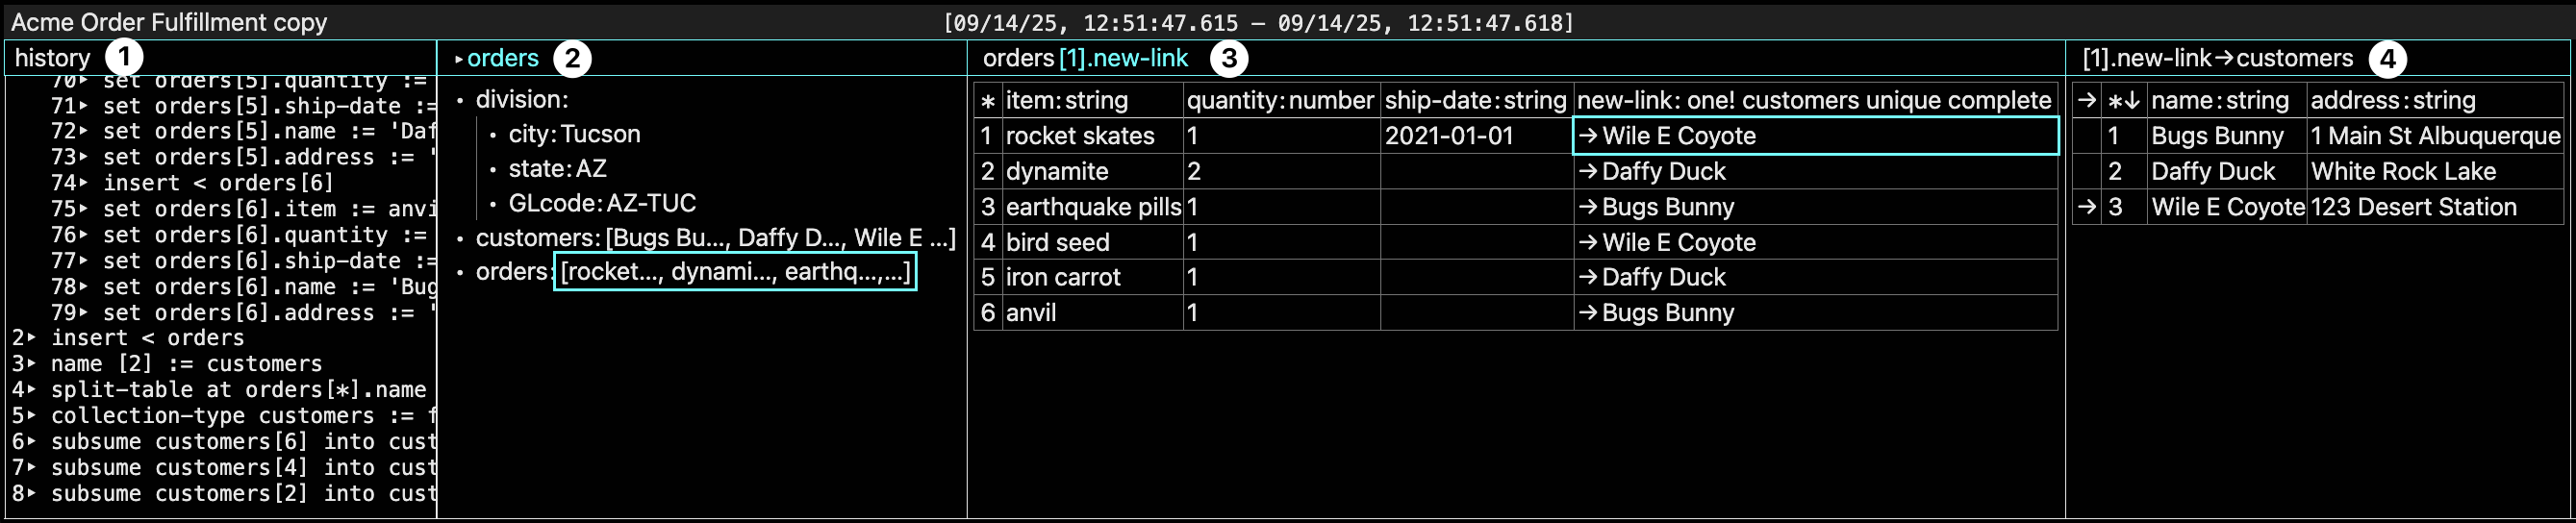
\includegraphics[width=\textwidth]{GUInumbered.png}
\caption{A selection is a path through Miller columns containing indented outlines and flat tables.}
\label{fig:GUI}
\end{figure}

\begin{figure}
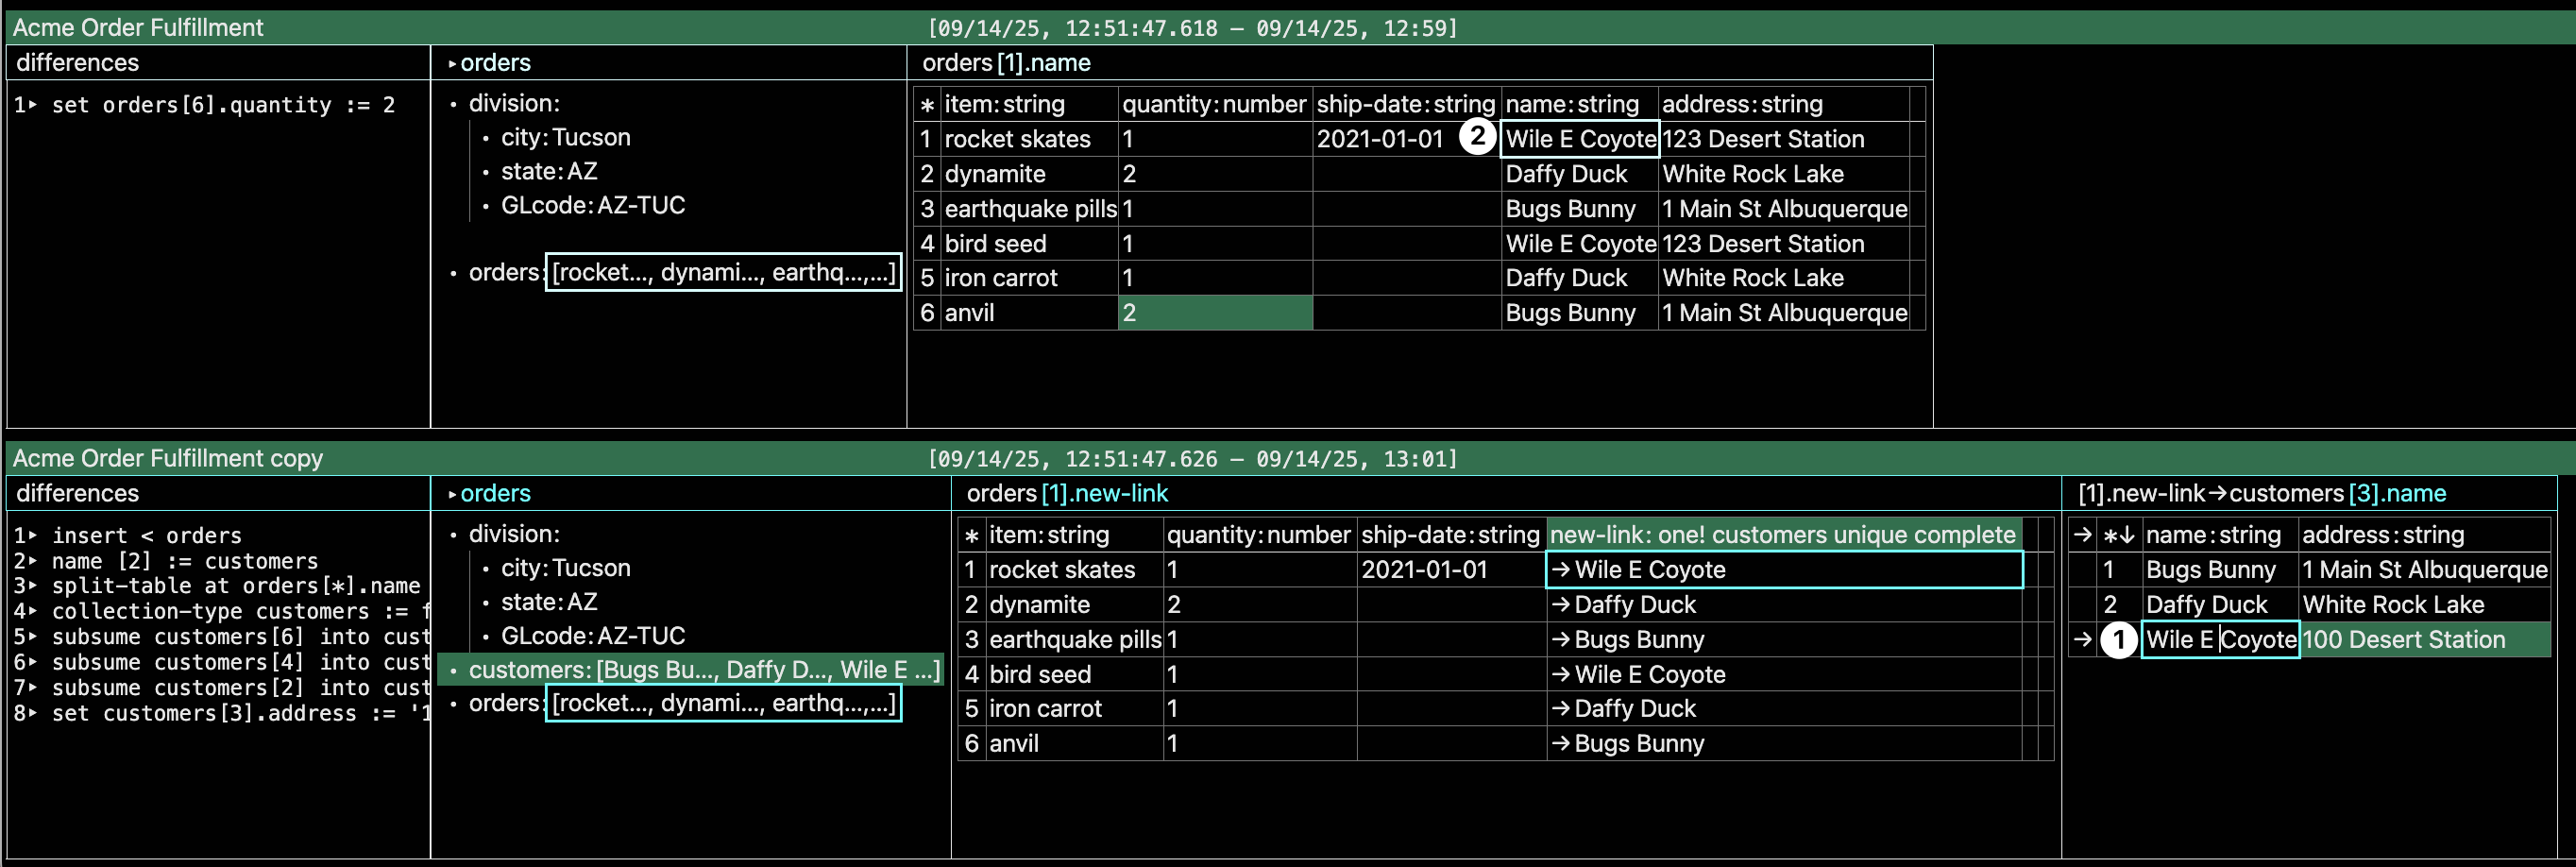
\includegraphics[width=\textwidth]{DiffNumbered.png}
\caption{A diff is displayed across a split screen with coordinated selection.}
\label{fig:Diff}
\end{figure}

\circledtextset{resize=real, charf=\LARGE\sffamily}
Figure~\ref{fig:GUI} displays a screen shot of the UI. \circledtext{1} The left hand column shows the history of operations on this database. History sidebars are a common technique but we were particularly inspired by Wrangler~\cite{kandel11}.

The three columns to the right are Miller columns~\cite{miller-columns} that display a path drilling into and across nested data structures. Usually Miller columns display a simple list, as in the MacOS Finder column view of directories. We elaborate that convention to show in each column either an indented outline or a flat table. Nested structures are indicated with summaries that when clicked open a new column to the right. Cyan outlines show the selected path through the columns. \circledtext{2} is the top-level structure of this document. \circledtext{3} is the \textsf{orders} table within it. The user has selected a link to the \textsf{customers} table, which is opened in the column \circledtext{4}. Selection not only drills into nested structures but also follows links crossing the hierarchy, as if the target table of the link was nested inside it. This design was inspired as a reaction to Ultorg~\cite{bakke:phdthesis, ultorg} which uses nested tables to represent queries crossing a flat relational database. Ultorg provides a single view of a nested structure whereas our use of Miller columns provides only a view of the context of a path within the structure. The compensation for that restriction is that each column contains a visually simpler and context-independent layout, keeping neighbors at each level adjacent to each other rather than being splayed across lower layers.

Figure~\ref{fig:Diff} displays our representation of diffs. The challege is that Operational Differencing can do fine-grained comparisons across schema changes. We split the screen in half vertically to compare two databases. Here we are displaying the differences due to database normalization between Figure~\ref{fig:tables-single} in the top half and Figure~\ref{fig:tables-dedup} in the bottom half. Differences on each side are given a green background, and the context menu on them provides a command to transfer that difference to the other side.

However the tricky problem is not showing the differences but showing what is the same across complex structural transformations.
We use \textit{coordinated selection}:  At \circledtext{1} the cyan outline indicates we have selected the \textsf{customers} table cell containing \textsf{Wile E Coyote}. At \circledtext{2} the corresponding cell in the other database has been outlined in white, even though it is in the \textsf{orders} table. We automatically compute the corresponding location of the selection by transfering a \textsf{noop} operation to the other side.

We first tried conventional representations of textual diffs, both side-by-side and interleaved (AKA unified). They have the advantage of keeping corresponding locations close to each other on screen, but only when the differences are limited to inserting and deleting lines of text. They did not adapt well to complex data structures and complex structural transformations. Our split-screen approach handles these cases as well, and has the advantage that the diff view keeps the layout of the data the same as in a normal view.




\section{Discussion}

% VC for everything, all the way down and up, Lisp redux
% full unified QL/PL with VC semantics, test, supply chain, deployment

%   \item If we are allowed to speculate, could we get the benefits of version control even at runtime? Could a replay debugger~\cite{Sundmark02, ocallahan16} let us step back in time, hot-patch a change, then roll foward and see the diffs? Could we explore and merge alternative runtime states~\cite{warth11}?
% DevOps~\cite{kim2022devops} would benefit from applying version control to migrating databases, or rebuilding containers, or updating software dependencies.

% eval: challenge problems, playable demo
% tech dims https://tomasp.net/techdims/#footer=index,navigation;left=catalogue,list;top=catalogue,index

% pros and cons
% con: need structural editor for code, or infer structure changes using known technique
% con: realtionship refactorings have been difficult, prob not right. family collapse not right
% design alternatives for relational actions.
% convergent evolution of insertions - move
% Need a rule spec language.
% transfer laws unclear
% We defer scaling issues to future work, focusing at first on small-scale data.
% query/formula editing
% structure editor
% We are exploring what is possible with an operation-based approach while defering the concerns of efficiency and interoperability.

% Does query rewriting hold up? Frankly this solution seems a bit too easy---we wonder if it will hold up as we fill out the capabilities of the query language.

% evalueate against existing techniques for schema evolution and version control. Or does that go in related work?


\section{Related Work}

% tribute to primary inspirations. wrangler, ultorg, lenses, refactoring DBs, SMOs, BiDel, Cambria [UVC?]
% git as anti-inspiration

% actually related work:
% Alex's worlds. Roly. Ask them for comment?
% Challenge problem paper.
% I&S: cambria, peritext, universal version control
% Braid time machine https://braid.org/time-machines

% cite hatra/paint papers!

% \subsection{Version Control}\label{VC}

% git, darcs, pijul

% git is the most established tool for change management but is also the source of much discontent. Pull refs from schema change paper. santiago's stuff. intentional?

% Understanding Version Control as Material Interaction with Quickpose
% https://dl.acm.org/doi/10.1145/3544548.3581394

% \subsection{The Impedance Mismatch Problem} \label{impedance}

% orthogonal persistence, ORMs, Linq, single tier (Tier, hop), naked objects, DBOS, durable computation

% \subsection{PL State Management}\label{PLstate}

% FP: Monads, Lenses

% Imperative: immutable, React state menagement

% Remark: lenses and state libraries
% Built in Mutable structure semantics?
% Pure FP uses lenses
% Imperative langs put it in libraries “immutable data” libraries and “reactive state management” libraries have cursors/paths (check immutable.js)
% We just add a path to values and build it into basic semantics
% Value + Path = context, pointed value, ?? “call-by-context”?
% Note UI manifest selection


% \subsection{OT}\label{OT}
% https://en.wikipedia.org/wiki/Operational_transformation
% inclusion/exclusion transform
% https://cedanet.com.au/ceda/ot/ot-control/
% forward/backward transposition %https://ieeexplore.ieee.org/document/655755

% \subsection{CRDT}\label{CRDT}

% \subsection{Schema Evolution}\label{schema-evolution}
% copy from challenge problems paper

% \citet{ambler06} propose in \textit{Refactoring Databases} the \textit{Split Table} refactoring and sketch the SQL needed. \citet(curino08) include \textit{Decompose Table} in a set of \textit{Schema Modification Operations} that automate evolutions. In our example these actions would split out the \textit{name} and \textit{address} columns into a new \textit{Customers} table and add a \textit{order} column as a \textit{foreign key} copying the \textit{primary key} of the order. But that does not solve the problem---we still have duplicate customers.
% BiDEL is only thing that solves problem

\printbibliography

\end{document}

% Local Variables:
% TeX-engine: luatex
% End:
